\documentclass{beamer}
\usepackage[utf8]{inputenc}
\usepackage{fourier}

\usepackage{amsfonts}
\usepackage{amsmath}		
\usepackage{amssymb}
\usepackage{beamerthemesplit}
\usepackage{bezier}
\usepackage{float}
\usepackage{hyperref}
\usepackage{longtable}
\usepackage{makeidx}
\usepackage{rotating}
\usepackage{wrapfig}
\usepackage{multirow}
\usepackage{pgf}
\usepackage{ragged2e}

\usetheme{Madrid}
\usefonttheme{serif}
\usecolortheme{default}

\graphicspath{ {../HCEP-50K-figures/} }

\title[Learning Molecular Representation]{Learning Molecular Representation}
\author[Hy \& Nguyen]{Hy Truong Son, Nguyen Duc Hai \\ Advisor: Prof. Risi Kondor}
\institute[UChicago]{The University of Chicago}
\date{December 2017}

\begin{document}

\logo{
\includegraphics[height=0.5cm]{Logo.jpg}}

\frame{\titlepage}

\begin{frame}
\frametitle{Harvard Clean Energy Project Dataset (HCEP)}
\begin{justify}
SMILES: C1C=CC=C1c1cc2[Se]c3c4occc4c4nsnc4c3c2cn1 \\
Power Conversion Efficiency (PCE, range 0 - 11): 5.16195
\begin{center}
	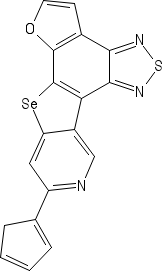
\includegraphics[scale=0.25]{sketcher}
	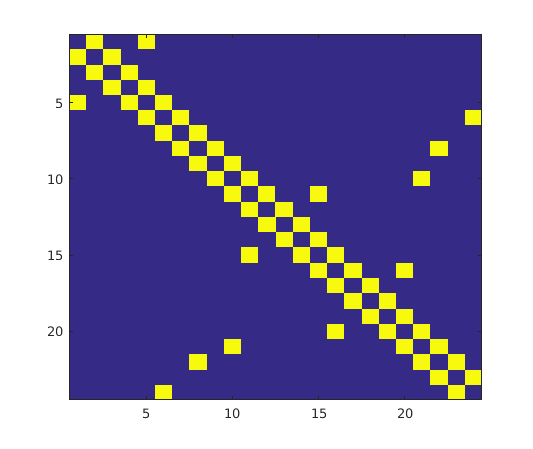
\includegraphics[scale=0.25]{adjacency}
\end{center}
\begin{center}
$C_{18}H_9N_3OSSe$ \ \ \ \ \ \ Adjacency matrix
\end{center}
\end{justify}
\end{frame}

\begin{frame}
\frametitle{dK-Series Algorithms (2)}
\begin{justify}
Reference: 
\begin{center}
\textbf{Systematic Topology Analysis and Generation Using Degree Correlations} \\ ACM SIGCOMM 2006
\end{center}
Algorithm:
\begin{enumerate}
	\item Extract all subgraphs of size $d$ in a molecular graph.
	\item Classify each subgraph as 1 element of the set of non-isomorphic graphs of size $d$.
	\item Based on the subgraph classification, we build the frequency vector (probability distribution) and use the frequency vector as the molecular graph representation. 
\end{enumerate}
Remark: Instead of using vertex degree, we use atomic types (for example, Carbon - C, Hydrogen - H, etc.).
\end{justify}
\end{frame}

\begin{frame}
\frametitle{Results \& Future Plan}
\begin{justify}
Results of using Linear Regression on dK-features:
\begin{center}
\begin{tabular}{|| c | c | c ||} 
\hline
& Test MAE & Test RMSE \\
\hline
$d = 1$ & 1.492278 & 3.457323 \\
\hline
$d = 2$ & 1.255755 & 2.545540 \\
\hline
$d = 3$ & 1.130819 & 2.194515 \\
\hline 
$d = 4$ & \textbf{1.025007} & \textbf{1.774689} \\
\hline
\end{tabular}
\end{center}
Next steps:
\begin{enumerate}
\item Apply more physical features rather than just atomic types
\item Apply state-of-the-art graph neural networks in learning molecular representations
\item Test on other molecular datasets
\end{enumerate}
\end{justify}
\end{frame}

\begin{frame}
\frametitle{}
\begin{center}
{\Large Thank you very much for your attention!}
\end{center}
\end{frame}

\begin{frame}
\frametitle{Q \& A}
\begin{justify}
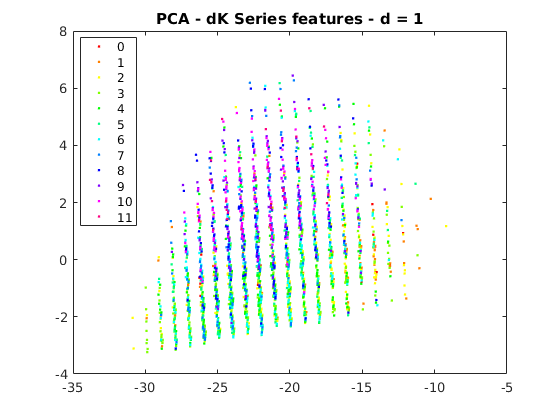
\includegraphics[scale=0.2]{d1-PCA}
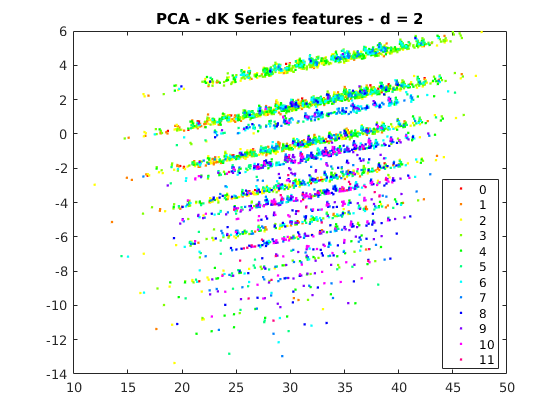
\includegraphics[scale=0.2]{d2-PCA}
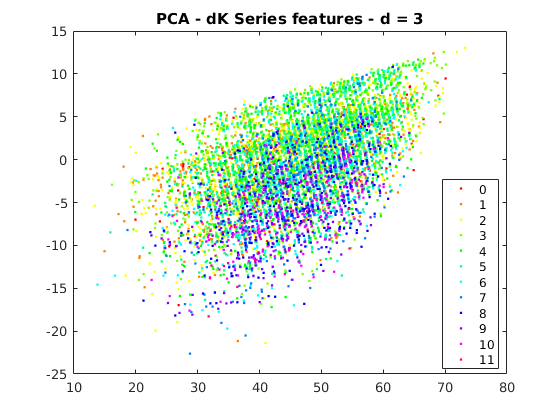
\includegraphics[scale=0.2]{d3-PCA}
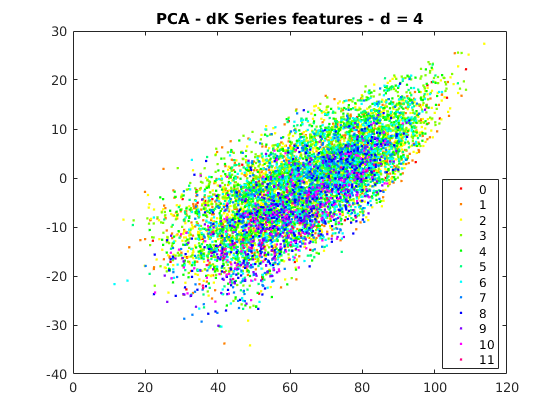
\includegraphics[scale=0.2]{d4-PCA} \\
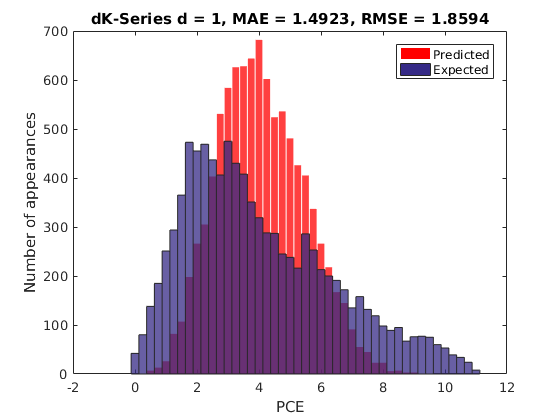
\includegraphics[scale=0.2]{d1}
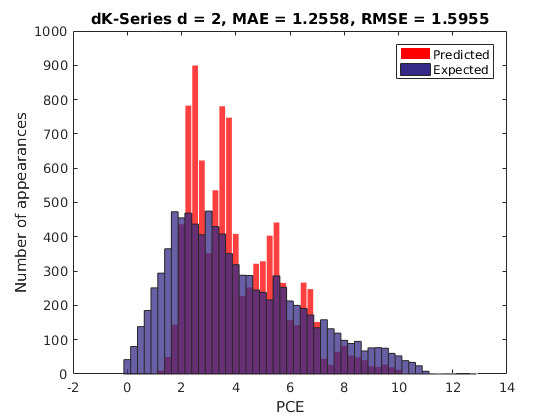
\includegraphics[scale=0.2]{d2}
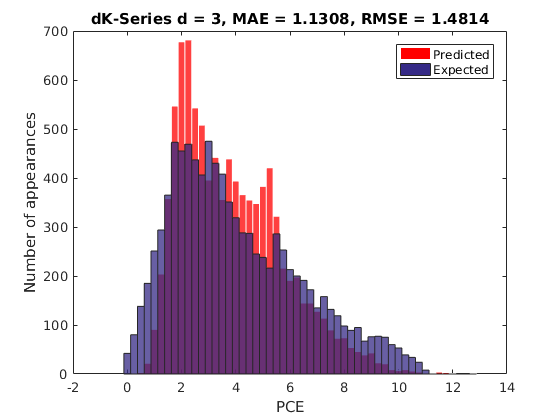
\includegraphics[scale=0.2]{d3}
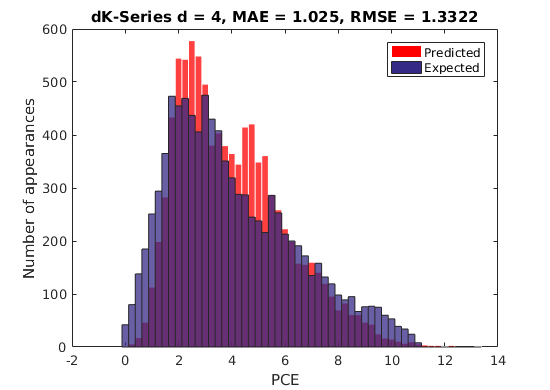
\includegraphics[scale=0.22]{d4}
\end{justify}
\begin{center}
\url{https://github.com/HyTruongSon/dk-series}
\end{center}
For more detail, read our paper \textbf{Covariant Compositional Networks For Learning Graphs} (ICLR 2018 - Workshop) [Kondor et. al.]
\end{frame}

\end{document}